\subsection{Descripción del problema.}

\vspace*{0.3cm}
\textbf{Introduccion} \newline
Como muchos saben en el ambito de las estadisticas, la mediana representa el valor de la variable en posicion central en un conjunto de datos ordenado.
Existen varios metodos para el calculo de la mediana, pero uno de los mas conocidos el siguiente.
Sean $\{x_1,x_2,x_3,...,x_n\}$ ordenadas en orden creciente, llamaremos $M_e$ a mediana del conjunto, pueden haber dos caso:

\begin{itemize}
    \item Si $n$ es impar, la mediana el valor ocupado en la posicion $(n+1)/2$, osea $M_e = x_{(n+1)/2}$.
    Ejemplo: tenemos 5 elementos ordenados $\{ 3,6,7,8,9 \}$ el valor central es el tercero, la mediana es elemento $M_e = 7$
    \item Si $n$ es par, la mediana es la suma de los elemento ocupados en la posicion $i/2$ y $i/2+1$ y luego dividir ese valor por 2, osea $ M_e = (x_{n/2} + x_{(n/2+1)})/2$.
    Ejemplo: Tenemos 6 datos ordenados $\{ 3,6,7,9,10,11 \}$ los dos valores para calcular la mediana son los $x_3=7$ y $x_4=9$, $ M_e = (7+9)/2 = 8$. 
\end{itemize}
En la \textbf{figura 3} tenemos unos graficos con las diferencias entre moda, mediana y media de una funcion arbitraria de densidad de probabilidad.	  
\begin{figure}[htb]
	\begin{center}
		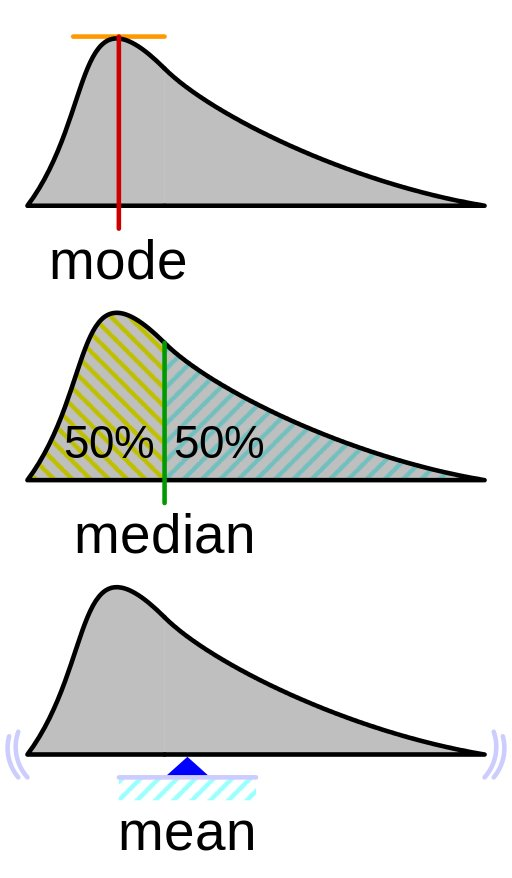
\includegraphics[scale=0.25]{imagenes/mediana.jpg}
	\end{center}
	\caption{Imagenes de la moda, mediana, media}
\end{figure}

\textbf{Problema} \newline

En nuestro problema nos han encomendado calcular y guardar las medianas parciales de una secuencia de numeros que no tine ningun orden fijo. \newline
Como por ejemplo: Nuestro secuencia de datos entrada(input) son \textbf{\{1,5,2,7,10\}}, las salida(output) debe ser \textbf{\{1,3,2,3,5\}},
en el cuadro de abajo los numeros marcados en negro son los numeros con los que calculo la mediana en ese instante. 

\begin{center}
   \begin{tabular}{| l | c | r | r |}
     \hline
     Nro de iteracion & 5 Nros entero(input)  &  Mediana en actual iteracion & Construccion de la secuencia solucion \\ \hline
     1 & \textbf{1} 5 2 7 10  & 1 & 1 \\ \hline 
     2 & \textbf{1 5} 2 7 10  & 3 & 1 3 \\ \hline 
     3 & \textbf{1 5 2} 7 10  & 2 & 1 3 2 \\ \hline 
     4 & \textbf{1 5 2 7} 10  & 3 & 1 3 2 3\\ \hline 
     5 & \textbf{1 5 2 7 10}  & 5 & 1 3 2 3 5\\ \hline 
     \hline
   \end{tabular}
\end{center} 

Veamos mas especificamente que quier decir el cuandro:.

\begin{itemize}
    \item En la itercion_1 calculo la mediana solamente con el elemento $1$,la mediana en ese instante es el $1$, mi secuencia solucion parcial queda $\{1\}$.
    \item En la itercion_2 calculo la mediana solamente con los elemento $\{1,5\}$, la mediana en ese instante es el $3$, mi secuencia solucion parcial queda $\{1,3\}$.
    \item En la itercion_3 calculo la mediana solamente con los elemento $\{1,5,2\}$, la mediana en ese instante es el $2$, mi secuencia solucion parcial queda $\{1,3,2\}$.
	\item y asi hasta llegar a la $5-esima$ iteracion, por consiguiente a la solucion.
\end{itemize}
%\begin{figure}[htb]
%  \begin{center}
%      \includegraphics[scale=0.25]{imagenes/ejemplo.jpg}
%  \end{center}
%  \caption{ejemplo}
%\end{figure}



\newpage
\subsection{Desarrollo de la idea y pseudocódigo.}

\vspace*{0.3cm}






Despues de cada numero de entrada se tiene que calcular la mediana en base a los numeros leidos hasta el momento,
entonces cuando llegamos al 1, solo tenemos a ese numero, y le resto de la secuencia no importa en el momento, entonces la secuencia de salida,
osea el secuencia de las medianas, se sabe que el i-esimo numero de la secuencia de salida, es la mediana, calculada entre el primer numero y el
i-esimo numero de entrada.

Entonces en base a ese problema, y que necesitamos tener un orden menor a $n^2$, encontramos una 
solucion que abarca una estructura de datos conocida, como es el Heap. En esta solucion usaremos dos heaps, uno ordenado de manera creciente,
y la otra de manera decreciente. Cuando hablo de manera creciente me refiero a que la raiz va a ser el menor numero, y que hacia abajo va a ir
teniendo numeros mayores o iguales. Ademas de usar 2 heaps para nuestra solucion, tambien estaremos usando un invariante entre estos dos heaps,
que tiene que cumplir, que en uno van a estar los numeros menores, y en el otro los mayores, y ademas de esto, otro invariante que el cardinal
de ambos no pueden tener una diferencia mayor a 1. Este invariante se usara para lograr calcular la mediana de forma rapida, ya que al tener el 
invariante de cardinalidad, sabemos que si uno de los dos tiene mayor cantidad de elementos, entonces su elemento, mayor o menor dependiendo de 
cual heap hablamos va a ser la mediana hasta ese momento, y si tienen la misma cardinalidad, va a ser el promedio de los dos numeros que 
predominan en cada uno de los heaps. Y esto se cumple solo porque esta el primer invariante de que en uno de los heaps estan los menores y en 
el otro los mayores.
Tambien tengo que aclarar que el heap de los numeros menores, va a tener a su mayor numero de raiz del heap, (osea como primer elemento), y que 
los numeros mayores van a tener a su menor elemento. En el codigo, de la solucion, la manera de mantener el invariante de que estan separados por
mayor y por menor, los heaps, se lo asegura jugando con el segundo invariante de cardinalidades. Se dice que cuando se tiene que agregar un numero
a un heap que tiene antes de agregarle, mas elementos que el otro, entonces hay que sacarle el primero( con primero me refiero a raiz de ese heap)
y pasarle ese numero al otro heap, y luego agregarle ese numero. De esta manera siempre se mantienen ambos invariantes, y para saber si se deberia
agregar en uno de los heaps o en el otro simplemente se fija, si el elemento a agregar, es mayor al menor de los mayores, o menor al mayor de
los menores.




\newpage
\subsection{Justificación de la resolución y demostración de correctitud.}

\vspace*{0.3cm}

%\textbf{completar!}
A continuacion vamos a justificar, porque se cumple el funcionamiento de el ejercicio 2.
Como hemos explicado anteriormente, tenemos dos colasPrioridad, que cumplen dos invariantes. HeapMenores, va a ser la ColaPrioridad que contenga a los elementos mas chicos leidos hasta el momento, y el HeapMayores va a ser la ColaPrioridad que contenga a los elementos mas grandes, leidos hasta el momento. \newline 

\textbf{Invariante: }
\begin{itemize}
    \item La cardinalidad de ambos, no tienen una diferencia mayor a 1. Con su cardinalidad me refiero a la cantidad de elementos que cada uno de las ColaPrioridad. %Desde ahora $#(HeapMenores)$ y $#(HeapMayores)$.
    \item El elemento mayor de la ColaPrioridad de los menores, va a contener un elemento, que sea menor o igual, al elemento menor del heap de los mayores.
\end{itemize}

En base a esto sacamos la conclucion de que, si la cardinalidad de ambas ColasPrioridad, son iguales, y son distintos de cero, entonces la cantidad de elementos es una cantidad par, por ende, segun la definicion de mediana, la mediana es el promedio de los dos elementos de los numeros ordenados, leidos hasta el momento. \newline
Y que si la cardinalidad es distinta, entonces la cantidad total de elementos leidos es impar, (esto se puede ver por el invariante de la diferencia), ya que: \newline

Si n es par, n+(n+1), es impar, ya que 2n es par, y un $par + 1$ es impar. \newline
Y lo mismo con n+(n-1), ya que 2n es par y un par -1 es impar.	\newline

Entonces por la definicion de mediana, la mediana es el elemento del medio de los numeros ordenados.

Ahora se analizara porque se cumple que el elemento del medio, en caso de que la cardinalidad total es impar, es el elemento primero, de la colaPrioridad que tenga la mayor cardinalidad.

Si miranmos una secuencia de numeros ordenados se va a poder ver claramente:
Supongamos que tengo la secuencia $\{1,2,3,4,5,6,7,8,9\}$, se puede ver que es el elemento $5$ es la mediana. \newline
Si se lo divide por menores y por mayores.

Por un lado tenemos los menores: $\{1,2,3,4\}$ y por otro los mayores, $\{6,7,8,9\}$
y luego el elemento del medio que podria ir en cualquiera de los dos. Por nuestra forma de implementarlo va a ir con los menores.
Entonces los menores, serian: $\{1,2,3,4,5\}$ y no solo que el 5 esta ahi, sino que es el elemento mayor, de los numeros chicos.
Si pondriamos al 5, con los mayores, este elemento seria el menor de ellos.
Nuestras ColasPrioridad estan ordenados de la siguiente manera: La ColaPrioiridad de los menores, tiene como primer elemento, al mayor. Y la ColaPrioridad de los mayores, tiene como primer elemento al menor.

Entonces si partimos una secuencia ordenada en dos partes iguales, los elementos del medio serian, el ultimo de la primera mitad, y el primero de la segunda, y esto es justamente lo que pasa con las ColasPrioiridad.
La ColaPrioiridad es nuestra forma de mantener ordenados los elementos, y el invariante de que su cardinalidad no tenga una diferencia mayor a 1, es la forma que hacemos para poder identificar rapido al elemento mediano.

Y la razon de que el elemento mediano es el primero(con primero revisar como esta hecha la ColaPrioridad) del que tenga mayor cardinalidad es porque:

Si tenemos n elementos, con n impar. Una ColaPriorodad va a contener (n-1)/2 elementos, y la otra (n-1)/2 + 1.
Podemos ver facilmente que si tenemos una secuencia de enteros ordenada, si vamos quitando el mayor y el menor cada vez, el elemento restante va a ser el elemento mediano.\newline
Vease este ejemplo simple:
Tengo la secuencia $\{1,2,3,4,5\}$  saco 1,5 $\rightarrow$  $\{2,3,4\}$  saco 2,4 $\rightarrow$ $\{3\}$ que es la mediana. \newline
Una vez que termina de recorrer todos los elementos de la entrada ,ahi el algoritmo devolvera la solucion(secuencia de medianas) y terminara.

\newpage
\subsection{Análisis de complejidad.}

\vspace*{0.3cm}

%\textbf{completar!}
Ahora que la forma de la solucion esta explicada, vamos a pasar a demostrar como es que cumple el orden de complejidad, menor a $n^2$.
Al tener dos conjuntos, basados en heap, y buscando en como esta implementado el heap que usamos de java, este explica que el orden cumple de 
agregar elementos en log $O(n)$, eliminar el primer elemento en $O(log(n))$, hacer un peek al primer elemento en $O(1)$ y buscar un elemento en $O(n)$,
pero esto no lo  hacemos nunca, porque no nos interesa todos los elementos en cada momento sino los primeros de cada heap.
\newline
Basandonos en que los heaps cumplen este orden pasamos a demostrar que nuestro codigo tambien cumple con este orden:
Nuestro codigo tiene un estilo de $while$, que es el que va a ir agarrando los numeros 1 por 1, esto se podria contar como un while de n numeros
suponiendo que n cumple que es la cantidad de numeros de entrada. Y luego, tiene los ifs correspondientes que son para verificar en cuales de
los casos explicados anteriormente cae el numero de entrada. Pero todo lo que hace en cada uno de los ifs, o el else, son simplemente verificar
en que caso cae que eso se cumple en $O(1)$ ya que son comparar numeros enteros, y luego en el peor de los casos tiene que sacar el primer elemento
de uno de los heaps (que eso se hace en $log (n)$ ) luego agregarlo en el otro heap (otro $log(n)$) y luego agregar ese elemento en su heap 
correspondiente ($log(n)$). Y esto cumple un orden de $3*(log(n))$ y si asumimos que el while es n veces, entonces son $3*n*log(n)$ que esta incluido
en el orden de $n*log(n)$. Y esto es exagerando un poco en realidad, porque cada uno de los heaps puede contener como mucho no $n$, sino $i/2$ elementos
con $i$ siendo la cantidad de numeros que ya leimos hasta el momento. Entonces en realidad el peor orden que puede tener nuestro ejercicio, 
es que siempre cuando son impares nuestro elemento caiga en el peor caso, que seria el de $3*log(i/2)$.



Entonces el peor caso es:

$ O(\sum_{i=1}^{n}3*log(i+1/2) + \sum_{i=1}^{n}3*log(i/2))= O(n*log(n)+3*n(log)) = O(n*log(n))$.

Que exagerando a los i por n, nos queda en el orden de $n*log(n)$.



\newpage
\subsection{Experimentación y gráficos.}

Para generar las instancias de toma de tiempos del problema 2 lo que hacemos es generar numeros aleatorios e ir guardandolos en un array hasta que este se llene, el tamaño del array se define segun el tamaño de la instancia que se quisiera. En el caso de lo que se quisiera fuera un peor caso, se generan numeros aleatorios, se le suma el anterior y se guarda en el array, ya que el peor caso es que los numeros vengan en forma creciente, teniedolos que guardar siempre en el heap de los mayores. Para en mejor caso se miraba cual tenia mas y se generaba un numero aleatorio que entrara en el heap de menor cantidad, si habia menos mayores se generaba un numero menor al minimo de los mayores y sino se generaba un numero y se le sumaba el mas grande de los chicos. En el caso de que tuvieran la misma cantidad se genera uno aleatorio y se guarda donde corresponda, en caso de que este entre el menor de los mayores y el mayor de los menores pasa a ser el mas grande de los menores. Para esto utilizamos la clase $ GeneradorInstancias $.

Se toman los tiempos igual que para el problema 1.
%Para tomar los tiempos pasamos 200 veces el mismo input(en el caso del ejercicio 3 hay que poner: pasamos 50 veces el mismo input, ya que tarda mucho en ejecutarse el programa con e grandes), y tomamos el promedio de los resultados que estuvieran un variacion estandar. Para ello filtramos los tiempos y nos quedamos con aquellos que estuvieran entre el promedio menos el desvio estandar y promedio mas el desvio estandar. El desvio estandar mide cuanto tienden a alejarse los resultados del promedio. Para calcular el desvio, primero tuvimos que calcular la varianza. Para obtener la varianza agarramos cada uno de los tiempos y  les restamos el promedio y lo elevamos al cuadrado, despues tomamos el promedio de esos resultados. Para terminar de calcular el desvio solo sacamos la raiz cuadrada de la varianza. Para esto utilizamos la clase $ Tiempos $.
%En el problema 1 se genero una secuencia de numeros aleatorios creciente, igual que en el peor caso del problema 2. dejando el tamaño del cable constante ya que este no afecta para las mediciones.


 En los siguientes gráficos tenemos los resultados obtenidos.

\begin{figure}[H]
  \begin{center}
      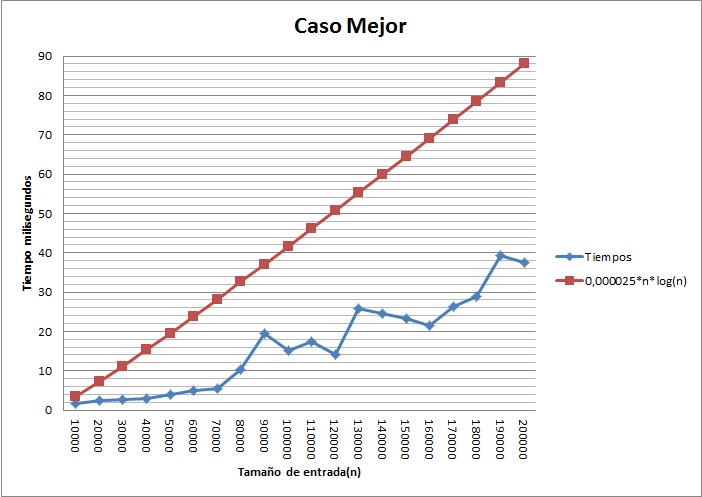
\includegraphics[scale=0.50]{imagenes/MejorCasoEj2.jpg}
  \end{center}
  \caption{ejemplo}
\end{figure}

El primer grafico del ejercicio 2, es el que compara al mejor caso con n*log(n), y en este grafico se puede ver claramente, que la curva de 
n*log(n) es una cota para los tiempos que se tomaron de lo que tarda en correr nuestro ejercicio para cotas cada vez mas grandes. Este grafico es importante mostrarlo, para que se vea que nuestro mejor caso, (que es mejor que el peor caso para todo n, visto del lado de complejidad de mejor y peor caso)
siempre esta acotado por n*log(n), que es siempre menor que n*n. Entonces aparte de la justificacion de la complejidad, habiendo tomado tiempos
no demuestra, pero apoya a la complejidad calculada.

\begin{figure}[H]
  \begin{center}
      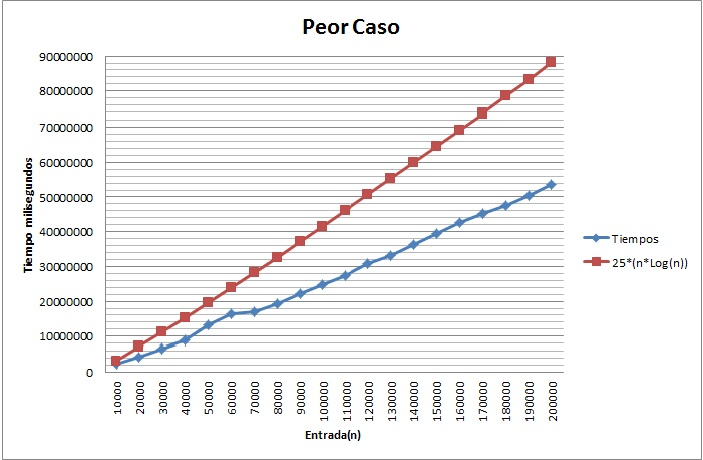
\includegraphics[scale=0.50]{imagenes/PeorCasoEj2.jpg}
  \end{center}
  \caption{ejemplo}
\end{figure}

El siguiente grafico, es el grafico de peor caso, comparado con n*log(n) que este es en realidad uno de los mas importantes, ya que tambien apoya nuestro calculo
de complejidad anterior, que decia que nuestro peor caso, para todo n = la sumatoria de i= 1 hasta n step 2 de log(i/2) + la sumatoria de i = 2 hasta n step 2 de 3*log(i/2)
Entonces al haber graficado n*log(n) por una constante, se puede ver que cae siempre por arriba de nuestros tiempos, y se puede ver que a la larga (mirando para n mayores)
la diferencia es cada vez mas grande.

\begin{figure}[H]
  \begin{center}
      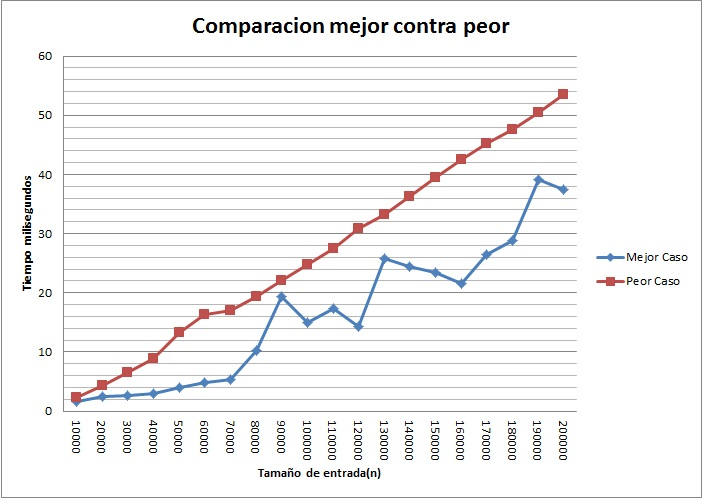
\includegraphics[scale=0.50]{imagenes/ComparacionEj2.jpg}
  \end{center}
  \caption{ejemplo}
\end{figure}

Y el grafico de mejor y peor caso, es simplemente para apoyar a la complejidad, ya que se puede ver facilmente que el mejor caso nunca puede ser mayor al peor.
Ya que la complejidad del mejor caso es la sumatoria de i = 1 hasta n de log(i/2) y la de peor caso mencionada varias veces es: la sumatoria de i= 1 hasta n step 2 de log(i/2) + la sumatoria de i = 2 hasta n step 2 de 3*log(i/2)
Entonces veremos que el grafico es coherente a lo recien dicho.



%\textbf{completar!}
\begin{figure}[H]
  \begin{center}
      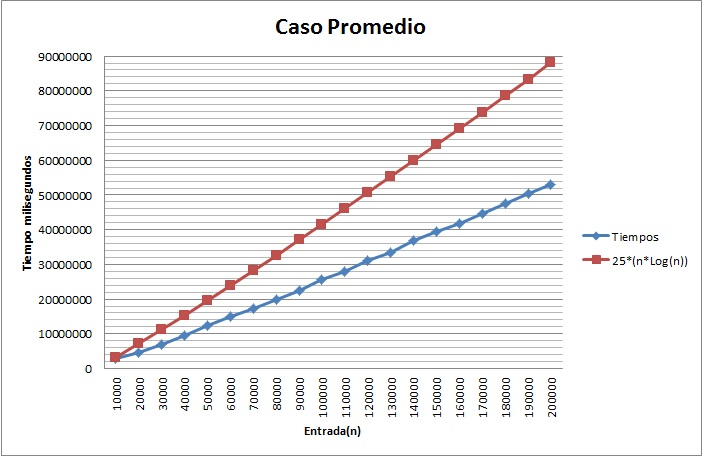
\includegraphics[scale=0.50]{imagenes/CasoPromedioEj2.jpg}
  \end{center}
  \caption{ejemplo}
\end{figure}

El ultimo grafico, es el del promedio, que este fue tomado agarrando numeros pseudoaleatorios, de la clase Random, de java. Este es el que probablemente
sea el mas parecido a como serian los tiempos tomados de cuando se use el programa, ya que si no buscas caer en un caso en particular, probablemente vayas cayendo en ambos casos, y 
no siempre en el mejor, ni siempre en el peor caso. Que como esta acotado por el peor caso, tambien es menor a n*log(n) y por consecuencia, a n al cuadrado.

\subsection{Validación}

Para validar el algoritmo, utilizamos casos de test, los cuales son una expansión de los test de la cátedra, para los cuales conocemos cual es la salida. En el archivo que contiene las instancias de entrada se llama $ Ej2\_validacion.in $, y los resultados esperados en $ Ej2\_validacion.out $.
